\documentclass[10pt]{article}

\usepackage[margin=0.75in]{geometry}
\usepackage{amsmath,amsthm,amssymb}
\usepackage{xcolor}
\usepackage{cancel}
\usepackage{graphicx}
\usepackage{changepage}
\usepackage{circuitikz}
\usepackage{minted}
\usepackage{pgfplots}
\usepackage{physics}
\usepackage{siunitx}
\usepackage[breakable]{tcolorbox}
\usepackage[inline]{enumitem}

\theoremstyle{definition}
\newtheorem{problem}{Problem}
\newtheorem{soln}{Solution}

\pgfplotsset{compat=newest}
\usetikzlibrary{lindenmayersystems}
\usetikzlibrary{arrows}

\definecolor{incolor}{HTML}{303F9F}
\definecolor{outcolor}{HTML}{D84315}
\definecolor{cellborder}{HTML}{CFCFCF}
\definecolor{cellbackground}{HTML}{F7F7F7}
\newcommand{\eq}{=}
\usetikzlibrary{positioning, fit, calc}
\pgfdeclarelayer{background}  
\pgfsetlayers{background,main}

\makeatletter
\newcommand{\boxspacing}{\kern\kvtcb@left@rule\kern\kvtcb@boxsep}
\makeatother
\newcommand{\prompt}[4]{
    \ttfamily\llap{{\color{#2}[#3]:\hspace{3pt}#4}}\vspace{-\baselineskip}
}

\newcommand{\thevenin}[2]{
  \begin{center}
    \begin{circuitikz} \draw
      (0,0) -- (2,0) to[battery1, l_=$V_{Th}\eq#1$] (2,2) 
      to[resistor, l_=$R_{Th}\eq#2$] (0,2)
      ;
      \draw [o-] (-.07,2.079);
      \draw [o-] (-.07,0.079);
    \end{circuitikz}
  \end{center}
}

\newcommand{\norton}[2]{
  \begin{center}
    \begin{circuitikz} \draw
      (0,0) -- (3,0) to[american current source, l_=$I_{N}\eq#1$] (3,2) -- (0,2) (2,0)
      to[resistor, l=$R_{N}\eq#2$] (2,2)
      ;
      \draw [o-] (-.07,2.079);
      \draw [o-] (-.07,0.079);
    \end{circuitikz}
  \end{center}
}

\newcommand{\highlight}[1]{\colorbox{yellow}{$\displaystyle #1$}}

\NewDocumentCommand{\evalat}{sO{\big}mm}{%
  \IfBooleanTF{#1}
   {\mleft. #3 \mright|_{#4}}
   {#3#2|_{#4}}%
}

\title{Math 2150: Assignment I}
\author{Jeremy Favro}
\date{\today}

\begin{document}

\maketitle
\noindent Note: I've kept $p$, $q$, and $r$ throughout my solutions and only substituted the actual numbers in at the end. This is because I find it easier,
especially when dealing with things that might cancel nicely, to deal with variables rather than the numbers they represent. In my case my
student number is 0805980 so $p=9$, $q=5$, and $r=22$.
\\
% PROBLEM 1
\begin{problem}
The primary objective of this exercise is to give you the opportunity to explore the effect
of damping and external forcing on mechanical vibration. The notes attached at the end of
this assignment provide the mathematical details of forced vibration which you may use to
contextualize your observations and discussions. You can use the SAGE commands and codes
I uploaded earlier on the blackboard to complete this assignment. I will also accept if you
use any other plotting or solution software. Your descriptions should be brief and precise. \\\\
\textbf{FORCED MECHANICHAL VIBRATIONS}
\\
Consider the forced mechanical vibration model of the spring-mass system that was discussed in the class,
\begin{equation}
  m\frac{d^2x}{dt^2}+b\frac{dx}{dt}+kx=f(t), \qquad x(0)=x_0, x^\prime(0)=x_1
\end{equation}
where $m$ is the mass of the object, $b$ is the damping constant, $k$ is the spring constant, and $f(t)$ is the applied
force acting on the spring-mass system at time $t$. Consider the special case where
\begin{equation}
  m=(p-q)^2,\quad k=q^2
\end{equation}
and
\begin{equation*}
  x_0=-1-\frac{q}{r}, \qquad x_1=1+\frac{p}{r}
\end{equation*}
\begin{enumerate}[label=(\alph*)]
  \item \textbf{UNDAMPED FORCE VIBRATION:} Consider the case where there is no damping ($b = 0$) and the applied force is given by
        \begin{equation}
          f(t)=p\sin\left(\omega t\right)+q\cos\left(\omega t\right)
        \end{equation}
        and with the initial conditions given above. Obtain \textbf{five plots} of the solution for each of the following $\omega$ values:
        \begin{equation}
          \omega=\sqrt{\frac{k}{m}}+\frac{i-3}{3},\qquad i=1,2,3,4,5
        \end{equation}
        The frequency $f_r=\frac{\omega}{2\pi}$ is called the \textbf{resonance frequency}. Describe the behaviour of the solutions
        at the resonance and the other frequencies.
  \item \textbf{DAMPED FREE VIBRATION:} Consider equation 1 with the damped free vibration case where $b \neq 0$ and $f (t) = 0$.
        For your particular $m$ and $k$ values, consider \textbf{three different} $b$ values in which the parameter
        \begin{equation}
          \Delta=b^2-4mk
        \end{equation}
        is
        \begin{enumerate}[label=\roman*.]
          \item Zero (Take $b=2q\left(p-q\right)$)
          \item Positive (Take $b=3q\left(p-q\right)$)
          \item Negative (Take $b=q\left(p-q\right)$)
        \end{enumerate}
        Obtain the \textbf{solution plots} for each of these cases. Describe the behaviour of the solutions.
  \item \textbf{DAMPED FORCED VIBRATION:} Consider equation 1 with
        \begin{equation}
          f(t)=\frac{r}{p}\sin\left(\gamma t\right)
        \end{equation}
        \begin{enumerate}[label=\roman*.]
          \item For the \textbf{underdamped oscillatory case of question 1(b)(iii) above,} obtain
                the \textbf{three plots} of the solution for
                \begin{equation}
                  b=q\left(p-q\right), \qquad \gamma=\sqrt{\frac{k}{m}-\frac{b^2}{2m^2}}, \qquad i=1,2,3
                \end{equation}
                Describe the behavior of the solutions that you observe from the plots.
          \item The amplitude of the oscillation in part 1(c)(i) is a product of the amplitude of the forcing, $\frac{r}{p}$, and the so called \textbf{Frequency gain} $M\left(\gamma\right)$ which is given by:
                \begin{equation}
                  M\left(\gamma\right)=\frac{1}{\sqrt{\left(k-m\gamma^2\right)^2+b^2\gamma^2}}
                \end{equation}
                The graph of $M\left(\gamma\right)$ is called the Frequency response curve. Graph each of the three frequency response curves
                (M as a function of $\gamma$ with the $\gamma$ axis ranging from 0 to 4 for the three different values $b$ used in question \#1(b) above. Describe your observations.
        \end{enumerate}
\end{enumerate}
\end{problem}
\newpage

\begin{soln} ~
  \begin{enumerate}[label=(\alph*)]
    \item At any frequency other than the resonance we see a chaotic increase and decrease in the amplitude of the oscillation.
          At resonance, the oscillation increases with time.
          \begin{tcolorbox}[breakable, size=fbox, boxrule=1pt, pad at break*=1mm,colback=cellbackground, colframe=cellborder]
            \prompt{In}{incolor}{1}{\boxspacing}
            \begin{minted}[breaklines, autogobble]{sage}
              clear_vars()
              import random
              from IPython.core.interactiveshell import InteractiveShell
              interactiveShell.ast_node_interactivity = "all"
              t = var('t')
              x = function('x')(t)

              q = 5
              p = 9
              r = 22

              m = (p-q)^2
              k = q^2
              d = diff(x, t)
              d2 = diff(d, t)

              plt = Graphics()
              for i in range(1,6):
                  omega = sqrt(k/m)+(i-3)/3
                  eqn = m*d2 + k*x == p*sin(omega*t) + q*cos(omega*t)
                  sol = desolve(eqn, x, ics=[0, -1-q/r, 1+p/r])
                  plt += plot(sol, 0, 10, legend_label=rf"$\omega={omega}$", color=random.choice(sorted(colors)))

              plt.legend(True)
              show(plt)
              \end{minted}
          \end{tcolorbox}
          \begin{tcolorbox}[breakable, size=fbox, boxrule=.5pt, pad at break*=1mm, opacityfill=0]
            \prompt{Out}{outcolor}{1}{\boxspacing}
            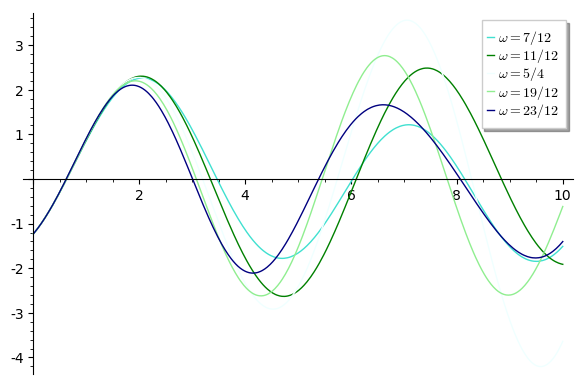
\includegraphics[scale=0.75]{G1.png}
          \end{tcolorbox}
          \newpage
    \item In the critically damped case we see a rapid non oscillating decay towards the steady state of the system. In the
          overdamped case we see a less rapid but still non oscillating decay towards the steady state of the system. In the underdamped case
          we see a slight oscillation that is dampened towards the steady state.
          \begin{tcolorbox}[breakable, size=fbox, boxrule=1pt, pad at break*=1mm,colback=cellbackground, colframe=cellborder]
            \prompt{In}{incolor}{2}{\boxspacing}
            \begin{minted}[breaklines, autogobble]{sage}
clear_vars()
t = var('t')
x = function('x')(t)

q = 5
p = 9
r = 22

m = (p-q)^2
k = q^2
d = diff(x, t)
d2 = diff(d, t)

plt = Graphics()
for i in range(1,4):
    b = i*((p-q)*q)
    eqn = m*d2 + b*d+ k*x == 0
    sol = desolve(eqn, x, ics=[0, -1-q/r, 1+p/r])
    plt += plot(sol, 0, 10, legend_label=rf"$b={b}$", color=random.choice(sorted(colors)))

plt.legend(True)
show(plt)
            \end{minted}
          \end{tcolorbox}
          \begin{tcolorbox}[breakable, size=fbox, boxrule=.5pt, pad at break*=1mm, opacityfill=0]
            \prompt{Out}{outcolor}{2}{\boxspacing}
            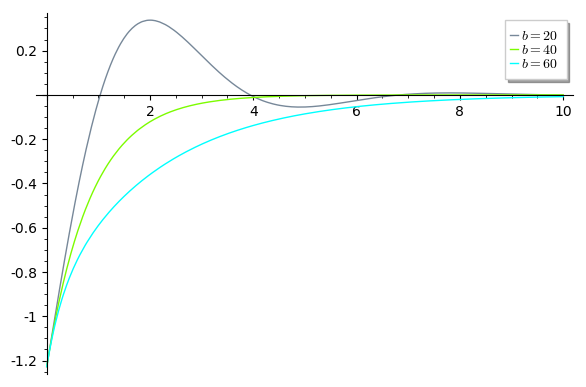
\includegraphics[scale=0.75]{G2.png}
          \end{tcolorbox}
          \newpage
    \item 
          \begin{enumerate}[label=\roman*.]
            \item For each case we see an initial (transient) oscillation which is quickly damped out towards the steady-state solution created by the driving oscillation.
            \begin{tcolorbox}[breakable, size=fbox, boxrule=1pt, pad at break*=1mm,colback=cellbackground, colframe=cellborder]
                    \prompt{In}{incolor}{3}{\boxspacing}
                    \begin{minted}[breaklines, autogobble]{sage}
clear_vars()
t = var('t')
x = function('x')(t)

q = 5
p = 9
r = 22

m = (p-q)^2
k = q^2
d = diff(x, t)
d2 = diff(d, t)

plt = Graphics()
for i in range(1,4):
    b = ((p-q)*q)
    gamma = sqrt((k/m)-((b^2)/(2*m^2)))+(i-2)/2

    eqn = m*d2 + b*d+ k*x == (r/p)*sin(gamma*t)
    sol = desolve(eqn, x, ics=[0, -1-q/r, 1+p/r])
    plt += plot(sol, 0.01, 10, legend_label=rf"$\gamma={gamma}$", color=random.choice(sorted(colors)))
    
plt.legend(True)
show(plt)
                \end{minted}
                  \end{tcolorbox}
                  \begin{tcolorbox}[breakable, size=fbox, boxrule=.5pt, pad at break*=1mm, opacityfill=0]
                    \prompt{Out}{outcolor}{3}{\boxspacing}
                    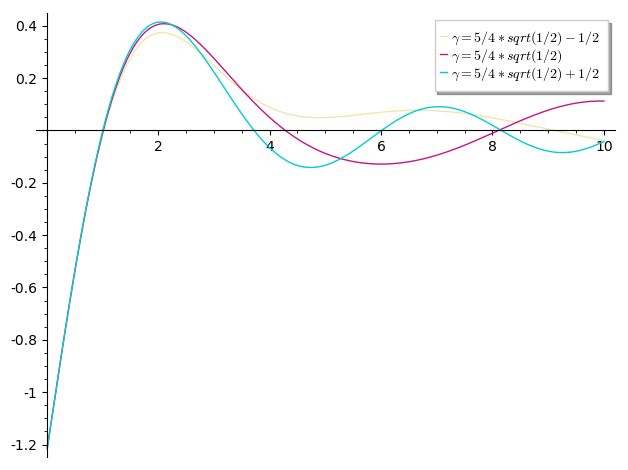
\includegraphics[scale=0.75]{G3.png}
                  \end{tcolorbox}
                  \newpage
            \item Here we observe that increased damping results in a lower overall frequency response. After some damping coefficient the resonant frequency
            is no longer apparent on the graph as the system is so highly damped that regardless of the frequency of the driving force there is minimal effect.
            \begin{tcolorbox}[breakable, size=fbox, boxrule=1pt, pad at break*=1mm,colback=cellbackground, colframe=cellborder]
                    \prompt{In}{incolor}{4}{\boxspacing}
                    \begin{minted}[breaklines, autogobble]{sage}
clear_vars()
t = var('t')
x = function('x')(t)

q = 5
p = 9
r = 22

m = (p-q)^2
k = q^2
d = diff(x, t)
d2 = diff(d, t)

plt_freq = Graphics()
gamma = var('gamma')
for i in range(1,4):
    b = i*((p-q)*q)
    M(gamma) = 1/(sqrt((k-m*gamma^2)^2+b^2*gamma^2))
    plt_freq += plot(M(gamma), 0, 4, legend_label=rf"$b={b}$", color=random.choice(sorted(colors))) 
    
plt_freq.legend(True)
show(plt_freq)
          \end{minted}
                  \end{tcolorbox}
                  \begin{tcolorbox}[breakable, size=fbox, boxrule=.5pt, pad at break*=1mm, opacityfill=0]
                    \prompt{Out}{outcolor}{4}{\boxspacing}
                    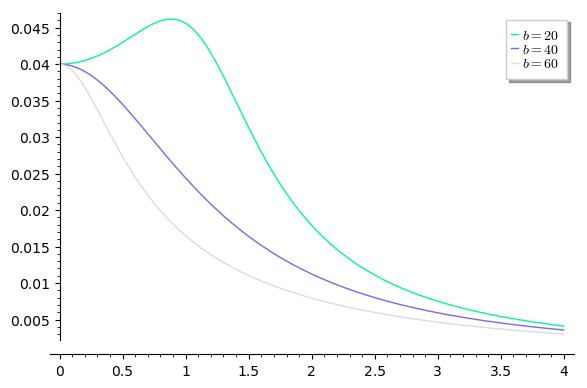
\includegraphics[scale=0.75]{G4.png}
                  \end{tcolorbox}
          \end{enumerate}
  \end{enumerate}
\end{soln}
\newpage

% PROBLEM 2
\begin{problem}
Solve the following differential equation using the method of undetermined coefficients.
$$\frac{d^2y}{dx^2}-2q\frac{dy}{dx}+q^2y=2q^2\left(q^2+4\right)^2\cos^2\left(x\right)+6pxe^{qx}+q^3x+(q^2+1)^2p\cos\left(x\right)$$
\end{problem}
\begin{soln} First we solve the homogeneous portion
  \begin{align*}
     & \frac{d^2y}{dx^2}-2q\frac{dy}{dx}+q^2y=0\rightsquigarrow y=e^{mx}                                                    \\
     & m^2-2qm+q^2=0 \implies m = \frac{2q\pm\sqrt{4q^2-4q^2}}{2} = q                                                       \\
     & \therefore y_h(x)=C_1e^{qx}+C_2xe^{qx} \text{ where } xe^{qx} \text{ is the result of reduction of order on } e^{qx} \\
  \end{align*}
  Then, using undetermined coefficients
  \begin{align*}
    y_p=                & A\cos\left(2x\right)+B\sin\left(2x\right)+Cx+D+x^2\left(Ex+F\right)e^{qx}+G\cos(x)+H\sin(x) \\
    y_p^\prime=         & -2A\sin(2x)+2B\cos(2x)+C+3Ex^2e^{qx}+qEx^3e^{qx}+2Fxe^{qx}+Fqx^2e^{qx}-G\sin(x)+H\cos(x)    \\
    y_p^{\prime\prime}= & -4A\cos(2x)-4B\sin(2x)+6Exe^{qx}+3Eqx^2e^{qx}+3Eqx^2e^{qx}+Eq^2x^3e^{qx}+2Fe^{qx}+          \\
                        & 2Fqxe^qx+2Fxe^{qx}+Fq^2x^2e^{qx}-G\cos(x)-H\sin(x)
  \end{align*}
  Which can then be plugged into the original differential equation in place of $y$, $y^\prime$, and $y^{\prime\prime}$
  \begin{align*}
     & -4A\cos(2x)-4B\sin(2x)+6Exe^{qx}+3Eqx^2e^{qx}+3Eqx^2e^{qx}+Eq^2x^3e^{qx}+2Fe^{qx}+2Fqxe^{qx}+2Fxe^{qx}+Fq^2x^2e^{qx} \\ &-G\cos(x)-H\sin(x)    \\
     & -2q\left[-2A\sin(2x)+2B\cos(2x)+C+3Ex^2e^{qx}+qEx^3e^{qx}+2Fxe^{qx}+Fqx^2e^{qx}-G\sin(x)+H\cos(x)\right]             \\
     & +q^2\left[A\cos\left(2x\right)+B\sin\left(2x\right)+Cx+D+x^2\left(Ex+F\right)e^{qx}+G\cos(x)+H\sin(x)\right]         \\
     & =q^2\left(q^2+4\right)^2+q^2\left(q^2+4\right)^2\cos\left(2x\right)+6pxe^{qx}+q^3x+(q^2+1)^2p\cos\left(x\right)
  \end{align*}
  Which when multiplied out yields
  \begin{align*}
     & -4A\cos(2x)-4B\sin(2x)+6Exe^{qx}+3Eqx^2e^{qx}+3Eqx^2e^{qx}+Eq^2x^3e^{qx}+2Fe^{qx}+2Fqxe^{qx}+2Fxe^{qx}+Fq^2x^2e^{qx}               \\
     & -G\cos(x)-H\sin(x) +4qA\sin(2x)-4qB\cos(2x)-2qC-6qEx^2e^{qx}-2q^2Ex^3e^{qx}-4qFxe^{qx}-2Fq^2x^2e^{qx}                              \\
     & +2qG\sin(x)-2qH\cos(x)+Aq^2\cos\left(2x\right)+Bq^2\sin\left(2x\right)+Cq^2x+D+Eq^2x^3e^{qx}+Fq^2x^2e^{qx}+q^2G\cos(x)+q^2H\sin(x) \\
     & =q^2\left(q^2+4\right)^2+q^2\left(q^2+4\right)^2\cos\left(2x\right)+6pxe^{qx}+q^3x+(q^2+1)^2p\cos\left(x\right)
  \end{align*}
  Which can be solved to determine the unknown coefficients
  \begin{align*}
     & -4B+4qA+Bq^2=0 \implies\frac{-4qA}{q^2-4}=B                                                                                \\
     & -4A-4qB+Aq^2=q^2\left(q^2+4\right)^2\implies\frac{q^2\left(q^2+4\right)^2}{q^2-4+\frac{16q^2}{q^2-4}}=A=525\implies B=-500 \\
     & Cq^2=q^3\implies C=q=5                                                                                                     \\
     & -2qC+D=q^2\left(q^2+4\right)^2\implies D=q^2\left(q^2+4\right)^2+2qC=21075                                                 \\
     & 2F=0\implies F=0                                                                                                           \\
     & 6E+2Fq+2F-4qF=6E=6p\implies E=p=9                                                                                          \\
     & -H+2qG+q^2H=0\implies \frac{-2qG}{q^2-1}=H                                                                                 \\
     & -G-2qH+q^2G=\left(q^2+1\right)^2p\implies G=\frac{\left(q^2+1\right)^2p}{\frac{4q^2}{q^2-1}-1+q^2}=216\implies H=-90       \\
  \end{align*}
  \begin{align*}
     & A=525   \\
     & B=-500  \\
     & C=5     \\
     & D=21075 \\
     & E=9     \\
     & F=0     \\
     & G=216   \\
     & H=-90   \\
  \end{align*}
  So,
  $$y_p=525\cos\left(2x\right)-500\sin\left(2x\right)+5x+21075+9x^3e^{5x}+216\cos(x)-90\sin(x)$$
  $$\therefore y=C_1e^{qx}+C_2xe^{qx}+525\cos\left(2x\right)-500\sin\left(2x\right)+5x+21075+9x^3e^{5x}+216\cos(x)-90\sin(x)$$
\end{soln}
\newpage

% PROBLEM 3
\begin{problem}
Solve the following differential equation using variation of parameters
$$qx^2\frac{d^2y}{dx^2}-9qx\frac{dy}{dx}+26qy=px^5\ln^2\left(x\right),\qquad x>0$$
\end{problem}
\begin{soln} First we solve the homogeneous portion
  \begin{align*}
     & qx^2\frac{d^2y}{dx^2}-9qx\frac{dy}{dx}+26qy=0 \rightsquigarrow y=x^m                                          \\
     & qx^2m^2x^{m-2}-9qxmx^{m-1}+26qx^m=0                                                                           \\
     & qm^2 -10qm+26q=0 \implies m=\frac{10q\pm\sqrt{100q^2-104q^2}}{2q}=5\pm i                                      \\
     & \therefore y_h(x)=C_1x^{5+i}+C_2x^{5-i}=x^5\left(C_3\cos\left(\ln(x)\right)+C_4\sin\left(\ln(x)\right)\right) \\
  \end{align*}
  Then, using variation of parameters
  $$y_p(x)=-y_1(x)\int\frac{g(x)y_2(x)}{W\left[y_1,y_2\right]}\,dx+y_2(x)\int\frac{g(x)y_1(x)}{W\left[y_1,y_2\right]}\,dx$$
  Where $g(x)=\frac{p}{q}x^3\ln^2\left(x\right)$ (the left hand side divided by $qx^2$).
  \begin{align*}
     & W\left[y_1,y_2\right]=
    \begin{vmatrix}
      y_1        & y_2        \\
      y_1^\prime & y_2^\prime
    \end{vmatrix}
    =
    \begin{vmatrix}
      x^5\cos\left(\ln(x)\right)                             & x^5\sin\left(\ln(x)\right)                             \\
      5x^4\cos\left(\ln(x)\right)-x^4\sin\left(\ln(x)\right) & 5x^4\sin\left(\ln(x)\right)+x^4\cos\left(\ln(x)\right)
    \end{vmatrix} \\
     & = \left[5x^4\sin\left(\ln(x)\right)+x^4\cos\left(\ln(x)\right)\right]x^5\cos\left(\ln(x)\right)
    -\left[5x^4\cos\left(\ln(x)\right)-x^4\sin\left(\ln(x)\right)\right]x^5\sin\left(\ln(x)\right)                  \\
     & = \cancel{5x^9\sin\left(\ln(x)\right)\cos\left(\ln(x)\right)}+x^9\cos^2\left(\ln(x)\right)
    \cancel{-5x^9\cos\left(\ln(x)\right)\sin\left(\ln(x)\right)} +x^9\sin^2\left(\ln(x)\right)                      \\
     & = x^9\cos^2\left(\ln(x)\right)+x^9\sin^2\left(\ln(x)\right) = x^9
  \end{align*}
  So,
  \begin{align*}
     & y_p(x)=-x^5\cos\left(\ln(x)\right)\int\frac{px^{8}\ln^2\left(x\right)\sin\left(\ln(x)\right)}{qx^9}\,dx                                                                 \\
     & +x^5\sin\left(\ln(x)\right)\int\frac{px^{8}\ln^2\left(x\right)\cos\left(\ln(x)\right)}{qx^9}\,dx                                                                        \\
     & =-\frac{p}{q}x^5\cos\left(\ln(x)\right)\left[2\ln(x)\sin\left(\ln(x)\right)+\left(2-\ln^2(x)\right)\cos\left(\ln(x)\right)\right]                                       \\
     & +\frac{p}{q}x^5\sin\left(\ln(x)\right)\left[\left(\ln^2(x)-2\right)\sin\left(\ln(x)\right)+2\ln(x)\cos\left(\ln(x)\right)\right]                                        \\
     & =-\frac{p}{q}x^5\cos\left(\ln(x)\right)2\ln(x)\sin\left(\ln(x)\right)-\frac{p}{q}x^5\cos\left(\ln(x)\right)\left(2-\ln^2(x)\right)\cos\left(\ln(x)\right)               \\
     & +\frac{p}{q}x^5\sin\left(\ln(x)\right)\left(\ln^2(x)-2\right)\sin\left(\ln(x)\right)+\frac{p}{q}x^5\sin\left(\ln(x)\right)2\ln(x)\cos\left(\ln(x)\right)                \\
     & = -\frac{p}{q}x^5\cos\left(\ln(x)\right)\left(2-\ln^2(x)\right)\cos\left(\ln(x)\right)+\frac{p}{q}\sin\left(\ln(x)\right)\left(\ln^2(x)-2\right)\sin\left(\ln(x)\right) \\
     & -\frac{p}{q}x^5\left(2-\ln^2(x)\right)\cos^2\left(\ln(x)\right)+\frac{p}{q}\left(\ln^2(x)-2\right)\sin^2\left(\ln(x)\right)                                             \\
     & = \frac{p}{q}x^5\left[-2\cos^2\left(\ln(x)\right)+\ln^2(x)\cos^2\left(\ln(x)\right)+\ln^2(x)\sin^2\left(\ln(x)\right)-2\sin^2\left(\ln(x)\right)\right]                 \\
     & = \frac{p}{q}x^5\left[\ln^2(x)-2\right]                                                                                                                                 \\
  \end{align*}
  $$\therefore y(x)=x^5\left(C_3\cos\left(\ln(x)\right)+C_4\sin\left(\ln(x)\right)+\frac{9}{5}\left[\ln^2(x)-2\right]\right) $$
\end{soln}
\end{document}